\chapter{Resultados \label{chap:Resultados}}
%%%%%%%%%%%%%%%%%%%%%%%%%%%%%%%%%%%%%%%%%%%%%%%%%%%%%%%%%%%%%%%%%%
%%%%%%%%%%%%%%%%%%%%%%%%%%%%%%%%%%%%%%%%%%%%%%%%%%%%%%%%%%%%%%%%%%
\section{Ajuste de espectros}
\noindent Habiendo calculado y aplicado los valores de expectación, $\mu_{g}$ y $\mu_{bkg}$, para corregir la carga sobre los clusters y habiendo introducido el modelo de la colección parcial de carga, usado en los ajustes de los espectros, ya se pueden obtener los resultados derivados de las correcciones.

Los resultados que se presentan a continuación son tanto para el pico del flúor como los picos del aluminio. Para ambos casos se muestran los histogramas de carga con sus respectivos ajustes, utilizando el modelo descripto en la Capítulo \ref{chap:ModeloPCC}, para el caso en el que se aplicó el umbral \verb|EPIX=1.5| con las correcciones. Se presentan en tablas los resultados tanto para el primer cuadrante del sensor como para el tercer cuadrante, debido a que el segundo cuadrante no funciona correctamente y el cuarto cuadrante presenta muchas \textit{hot columns}.


%Para ambos casos se muestran los histogramas con sus respectivos ajustes para cada uno de los pasos del análisis con el fin de poder comparar los resultados de unos con otros: Primero utilizando el umbral \verb|EPIX=0.5|, luego aumentando el umbral a \verb|EPIX=1.5| sin aplicar las correcciones y, por último, los resultados con el umbral \verb|EPIX=1.5| aplicando las correcciones. Todos los resultados que se presentan son para el primer cuadrante del sensor.

%%%%%%%%%%%%%%%%%%%%%%%%%%%%%%%%%%%%%%%%%%%%%%%%%%%%%%%%%%%%%%%%%%
%%%%%%%%%%%%%%%%%%%%%%%%%%%%%%%%%%%%%%%%%%%%%%%%%%%%%%%%%%%%%%%%%%
\subsection{Aluminio}
\noindent En el gráfico de la Figura \ref{fig:Al_OHDU1_EPIX15_Corr} se puede ver el histograma de carga del aluminio con su ajuste, obtenido de los datos procesados con el umbral \verb|EPIX=1.5| y con las correcciones aplicadas. De este puede observarse la cola del ajuste a la izquierda de los picos debido a la incidencia de la colección parcial de carga. Se observa como este fenómeno produce un efecto sutilmente apreciable en el gráfico y es claro que no puede despreciarse. Por otro lado, los resultados para los tres pasos del análisis realizado, es decir, con el umbral original \verb|EPIX=0.5|, \verb|EPIX=1.5| y \verb|EPIX=1.5| con correcciones se condensan en la Tabla \ref{tab:Al_FanoEehOHDU1y3} y en los gráficos de la Figura \ref{fig:Al_mu_sigma_fano}.
\begin{table}[h]
\centering
\begin{tabular}{@{}ccccc@{}}
\toprule
                & \multicolumn{2}{c}{OHDU1}                 & \multicolumn{2}{c}{OHDU3}                 \\ \hline\hline
                & $F$                 & $\varepsilon_{\eh}$ & $F$                 & $\varepsilon_{\eh}$ \\
EPIX 0.5 & $0.1322 \pm 0.0022$ & $3.7141 \pm 0.0019$ & $0.1498 \pm 0.0101$ & $3.7209 \pm 0.0029$ \\ 
EPIX 1.5 & $0.1455 \pm 0.0098$ & $3.7379 \pm 0.0024$ & $0.1699 \pm 0.0150$ & $3.7419 \pm 0.0039$ \\ 
EPIX 1.5 Corr & $0.1464 \pm 0.0096$ & $3.7501 \pm 0.0006$ & $0.1504 \pm 0.0011$ & $3.7485 \pm 0.0039$ \\ \bottomrule \hline
\end{tabular}
\caption{tabla}
\label{tab:Al_FanoEehOHDU1y3}
\end{table}

\begin{figure}[h]
    \centering
        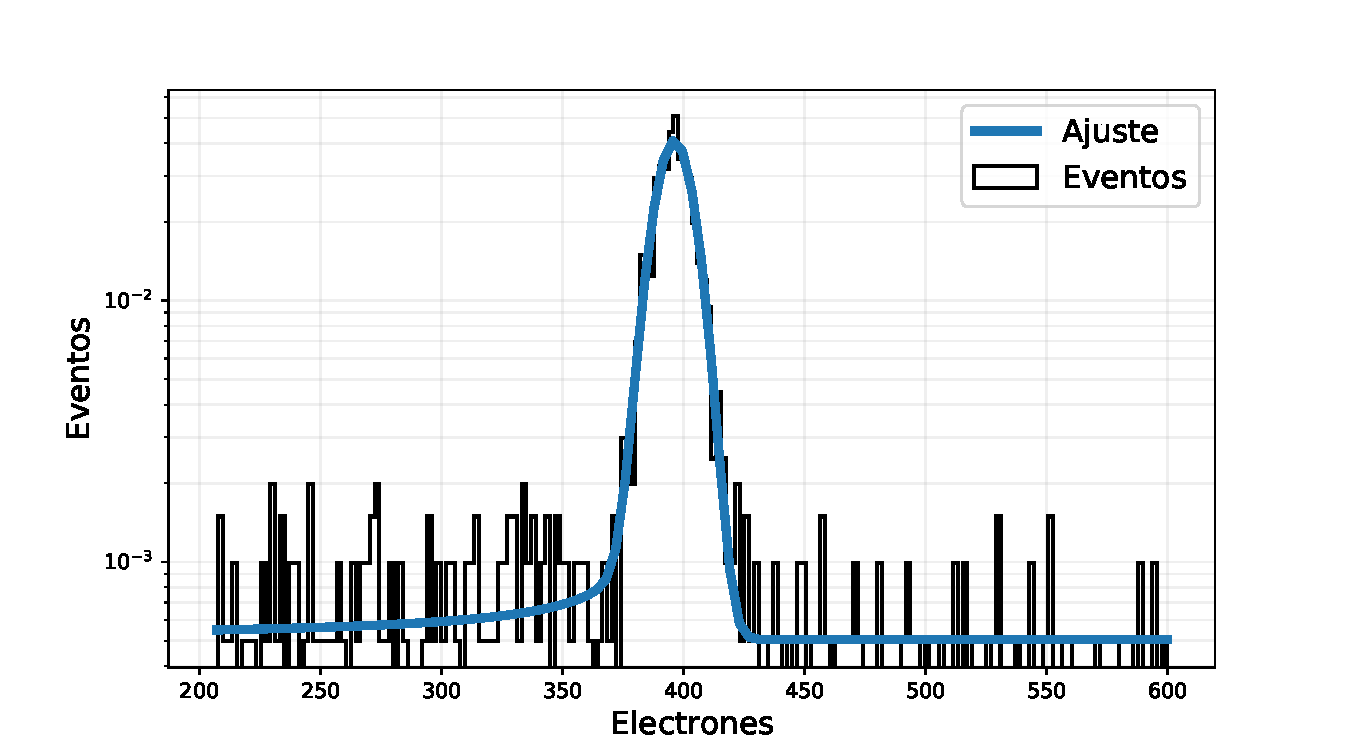
\includegraphics[scale=0.5]{Figs/HistFit_100c_EPIX15_OHDU1_Corr.pdf}
    \caption{\footnotesize{Histograma y ajuste del pico de los rayos $X$ del aluminio utilizando el modelo. El efecto de la colección parcial de carga es leve pero apreciable.}}
    \label{fig:Al_OHDU1_EPIX15_Corr}
\end{figure}

Por un lado se tiene que el valor del factor de Fano aumenta al pasar de \verb|EPIX=0.5| a \verb|EPIX=1.5|, al mismo tiempo que sus incertezas, tanto para el primer cuadrante como para el tercero, lo cual no era un resultado anticipable dado el aumento de estadística. El factor de Fano aumenta $\sim 10\,\%$ y su incerteza aumenta más de $4$ veces para el primer cuadrante, mientras que para el segundo el factor de Fano aumenta $\sim 12\,\%$y su incerteza un $\sim 50\,\%$.

\begin{figure}[h]
    \centering
        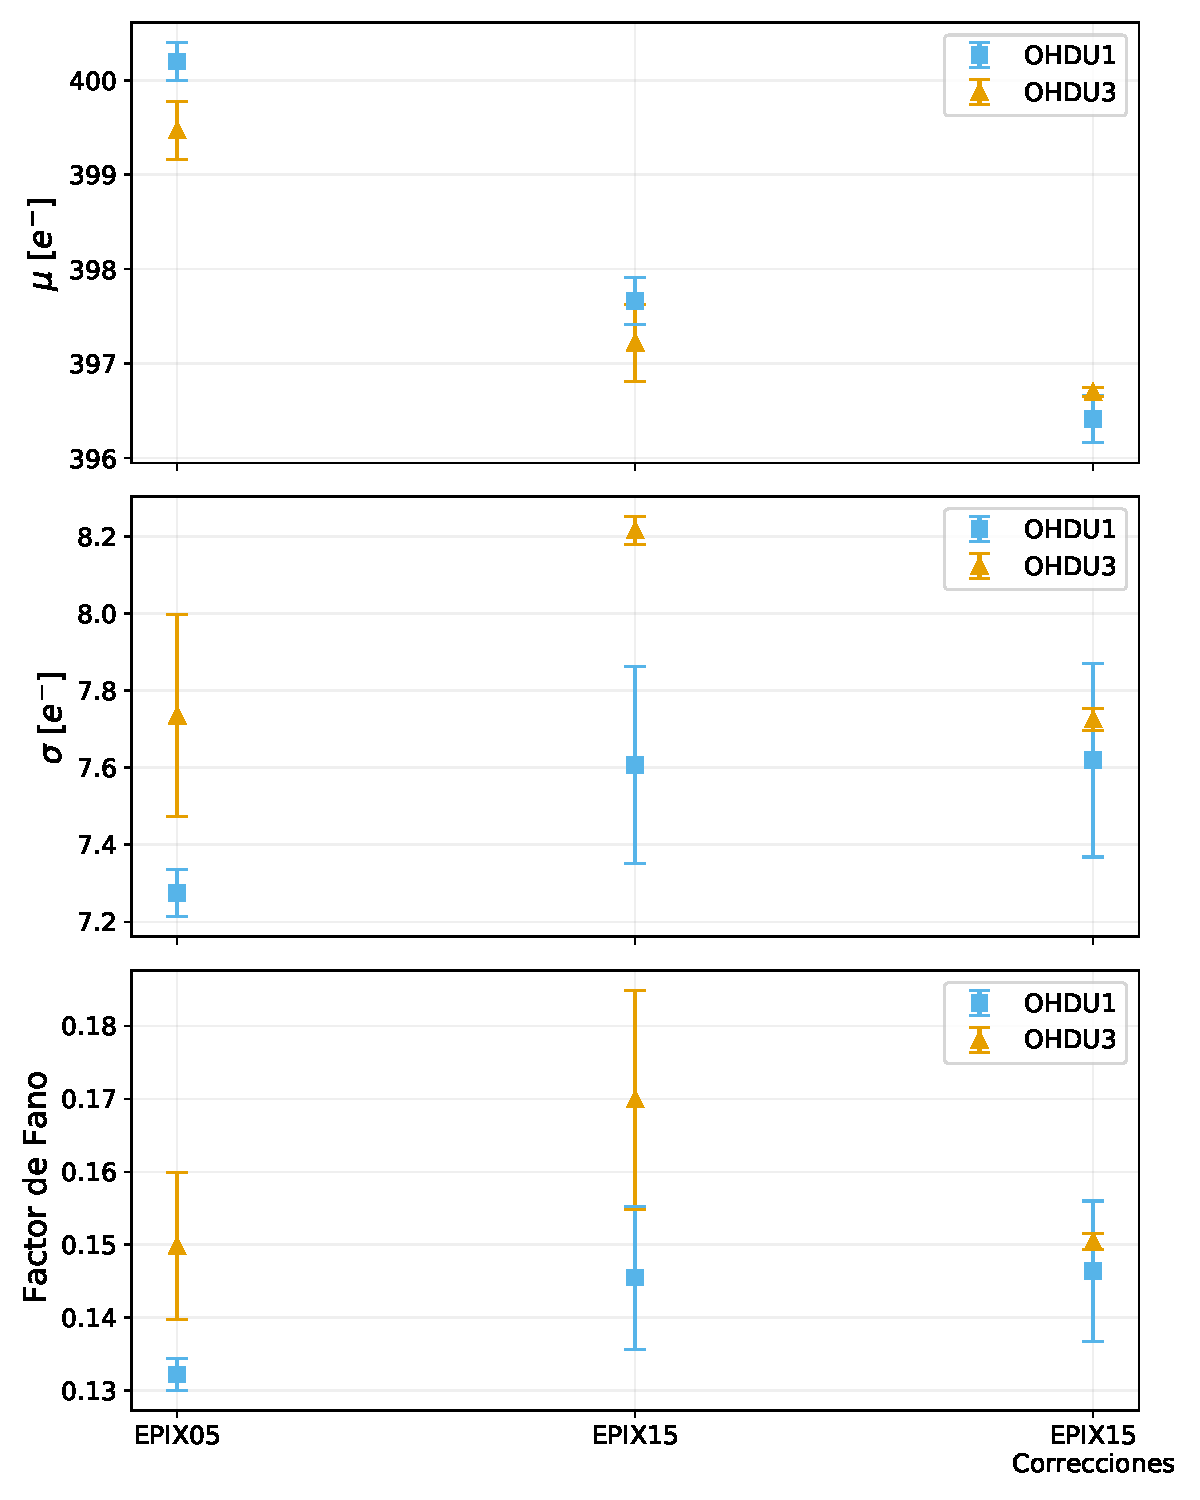
\includegraphics[scale=0.5]{Figs/Al_mu_sigma_fano.pdf}
    \caption{\footnotesize{Valores para las magnitudes relevantes para el factor de Fano, para los cuadrantes uno y tres, para los tres pasos de análisis implementados. Arriba: Valor medio del pico de rayos $X$ del aluminio; medio: Dispersión de los picos; abajo: factor de Fano. Se observa que la tendencia del factor de Fano sigue la misma tendencia de la dispersión.}}
    \label{fig:Al_mu_sigma_fano}
\end{figure}
Al aplicar las correcciones respecto al paso anterior lo que se obtiene es una ligera disminución del valor del Fano para el primer cuadrante, menor al $1\,\%$, y otra no tan ligera disminución para el tercero, cerda del $\sim 12\,\%$, donde curiosamente las incertezas no se comportan de la misma manera para ambos casos: Para el primer cuadrante la incerteza aumenta levemente, $\sim 3\,\%$, mientras que para el tercero disminuye muchísimo, mas del $\sim 95\,\%$. Todo esto puede verse con mayor claridad en el tercer gráfico de la Figura \ref{fig:Al_mu_sigma_fano}. Cabe destacar que los valores del factor de Fano para ambos cuadrantes se solapan con su error, de forma que los resultados para ambos cuadrantes resultan compatibles.

Es interesante notar que el aumento del factor de Fano al aplicar el umbral se debe a un aumento de la dispersión de los picos, $\sigma$, como se ve en el segundo gráfico de la Figura \ref{fig:Al_mu_sigma_fano}. Es decir, al aumentar la estadística también aumenta el ancho de los picos.

En cuanto a la energía de creación electrón-hueco, para cada paso del análisis su valor aumentó, como puede verse en el gráfico de la Figura \ref{fig:Al_energia_creacion_eh}. En este caso el aumento de la estadística y las correcciones implementadas compatibilizaron los resultados entre los dos cuadrantes dado que sus incertezas se solapan y sus valores absolutos difieren menos de $0.1\,\%$.
\begin{figure}[h]
    \centering
        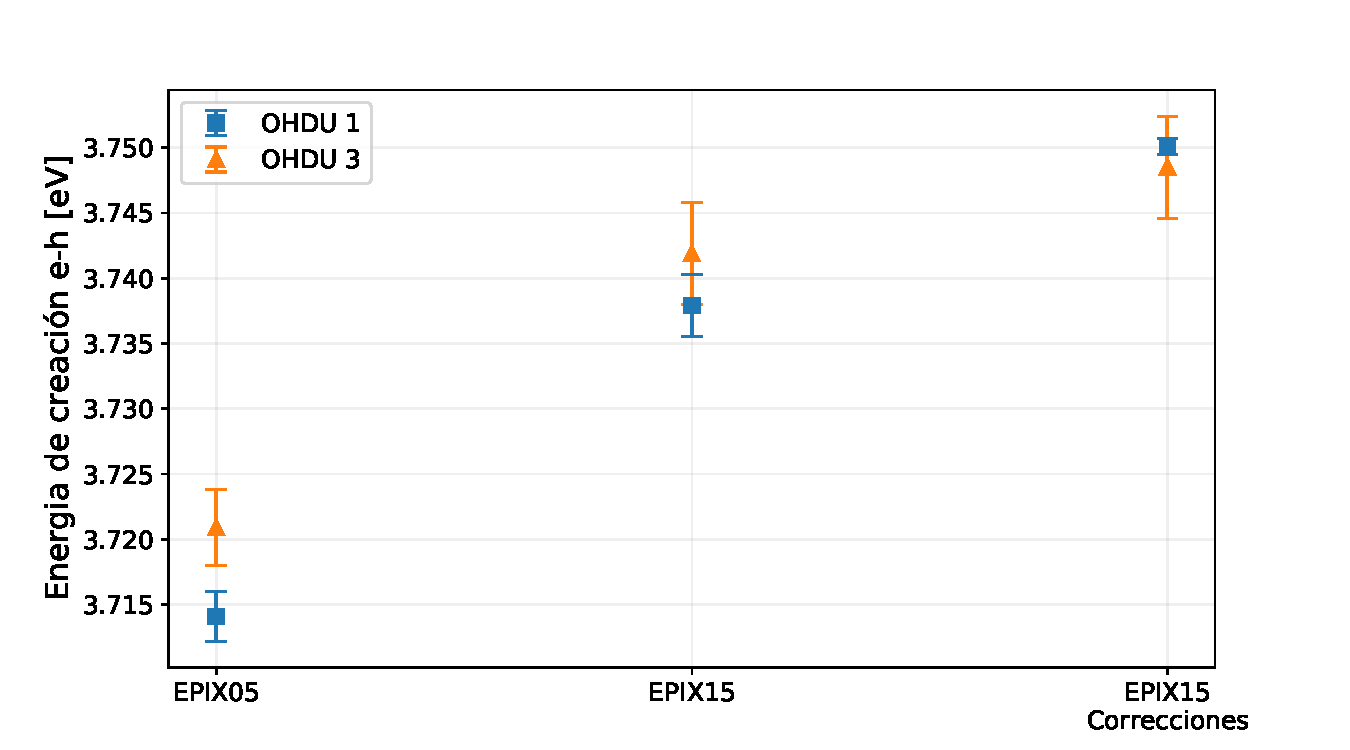
\includegraphics[scale=0.5]{Figs/Al_energia_creacion_eh.pdf}
    \caption{\footnotesize{asd.}}
    \label{fig:Al_energia_creacion_eh}
\end{figure}


\noindent Los valores del parámetro $\beta$, del cual puede obtenerse el tamaño de la región de PCC, junto con su error se determinaron utilizando el método de la máxima verosimilitud como se detalla en la sección \ref{sec:MaximaVerosimilitud}. De realizar este procedimiento se obtuvieron los gráficos de la verosimilitud que se ven en la Figuras \ref{fig:LL_beta_OHDU1} y \ref{fig:LL_beta_OHDU3} que se ajustaron con una función cuadrática de la cual se obtiene el valor de $\hat{\beta}$ que maximiza las curvas. En ambos casos se grafica la recta que se encuentra a una distancia $a=1/2$ por debajo del máximo y su intersección con la curva obtenida del barrido en $\beta$ para la verosimilitud, de donde se obtuvieron los intervalos $[0.00396, 0.01144]$ para el primer cuadrante y $[0.014152, 0.023138]$ para un $68.3\,\%$ de probabilidad de contener a $\beta$, para el primer y tercer cuadrante del sensor respectivamente.
\begin{figure}[H]
    \centering
        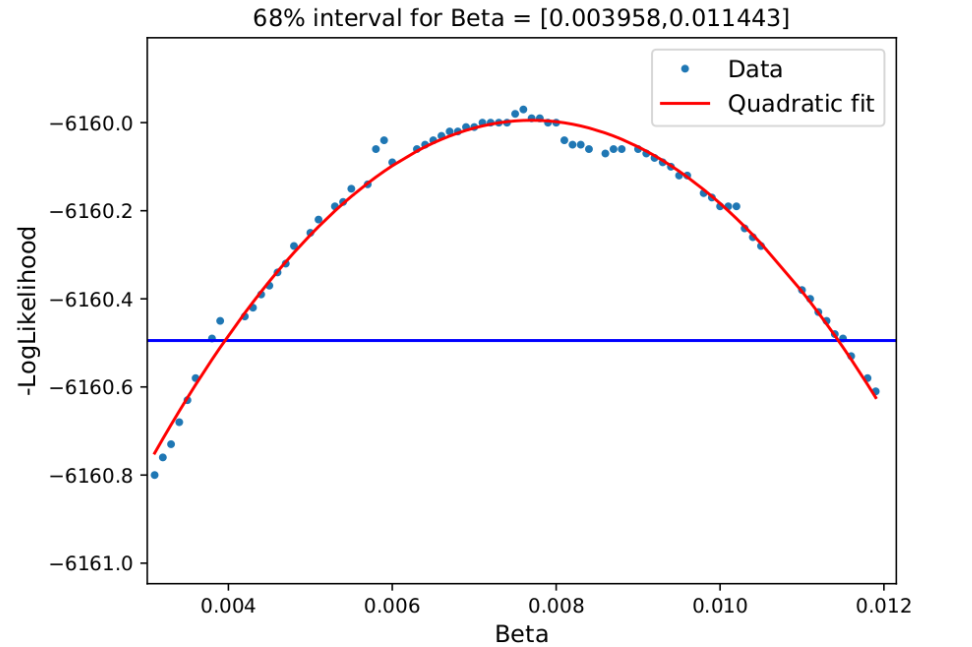
\includegraphics[scale=0.4]{pngs/LL_beta_OHDU1.png}
    \caption{\footnotesize{asd.}}
    \label{fig:LL_beta_OHDU1}
\end{figure}
\begin{figure}[H]
    \centering
        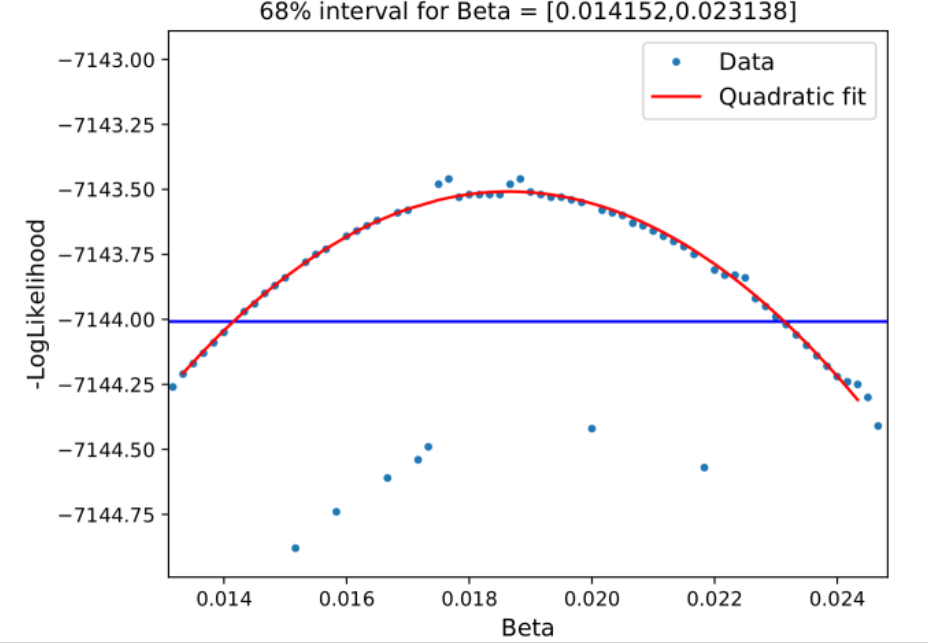
\includegraphics[scale=0.4]{pngs/LL_beta_OHDU3.png}
    \caption{\footnotesize{asd.}}
    \label{fig:LL_beta_OHDU3}
\end{figure}
La razón por la que se calcula el valor de $\beta$ y su intervalo es para conocer cuánto se extiende la región de PCC en el detector. Sabiendo que para el aluminio la distancia de atenuación de $8\,\si{\mu m}$, y para el valor de $\beta$ obtenido, se deriva que la extensión de la región de colección parcial de carga es de $\tau_{\scaleto{CCE}{4pt}} = algo \pm otra cosa$.

%%%%%%%%%%%%%%%%%%%%%%%%%%%%%%%%%%%%%%%%%%%%%%%%%%%%%%%%%%%%%%%%%%
%%%%%%%%%%%%%%%%%%%%%%%%%%%%%%%%%%%%%%%%%%%%%%%%%%%%%%%%%%%%%%%%%%
\subsection{Fluor}
\noindent La primera diferencia para el análisis de los resultados del flúor es que para su ajuste se utilizó el $\beta$ obtenido del método de maximización de la verosimilitud utilizado para el aluminio. No está de más recordar que esto es posible hacerlo porque del valor de $\beta$ se desprende directamente el valor del ancho de la región de PCC $\tau_{\scaleto{CCE}{4pt}}$ que es una característica del sensor. De esta forma, obteniendo el valor $\tau_{\scaleto{CCE}{4pt}}$ del valor de $\beta$ del aluminio y $\tau_{\scaleto{X}{4pt}}$ de tablas para el flúor, se desprende el $\beta$ utilizado para estos ajustes.

En la Figura \ref{fig:F_OHDU0_EPIX15conCorr} se tiene el histograma de carga para el pico de flúor con su respectivo ajuste, para el primer cuadrante del sensor y luego de aplicar el umbral \verb|EPIX=1.5| y las correcciones. Se observa como la colección parcial de carga afecta a estos picos de forma mucho más pronunciada que para el aluminio, formando colas a la izquierdo de estos. Esto es un resultado que se anticipaba en el Capítulo \ref{chap:ModeloPCC}, y que quiere decir que el valor de $\beta$ es mayor para el flúor.
\begin{figure}[h]
    \centering
    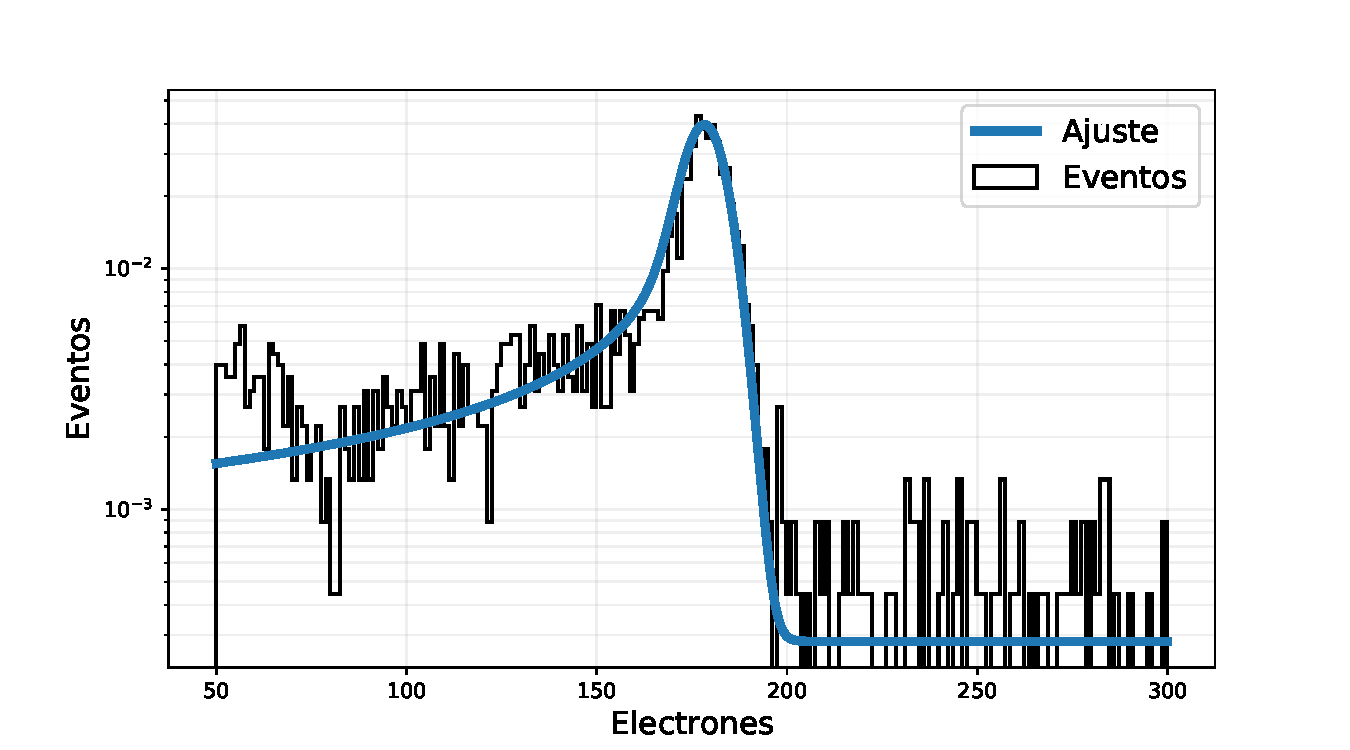
\includegraphics[scale=0.5]{Figs/HistFit_F_EPIX15_OHDU1_Corr.pdf}
    \caption{\footnotesize{\textbf{completar}}}
    \label{fig:F_OHDU0_EPIX15conCorr}
\end{figure}
En la Tabla \ref{tab:F_FanoEehOHDU1y3} se presentan los resultados para los tres pasos del análisis para los cuadrantes uno y tres.
\begin{table}[h]
\centering
\begin{tabular}{@{}ccccc@{}}
\toprule
                & \multicolumn{2}{c}{OHDU1}                 & \multicolumn{2}{c}{OHDU3}                 \\ \hline\hline
                & $F$                 & $\varepsilon_{\eh}$ & $F$                 & $\varepsilon_{\eh}$ \\
EPIX 0.5 & $0.1616 \pm 0.0128$ & $3.6963 \pm 0.0005$ & $0.1748 \pm 0.0138$ & $3.7211 \pm 0.0052$ \\ 
EPIX 1.5 & $0.1759 \pm 0.0169$ & $3.7726 \pm 0.0030$ & $0.1813 \pm 0.0179$ & $3.7802 \pm 0.0069$ \\ 
EPIX 1.5 Corr & $0.1648 \pm 0.0085$ & $3.7784 \pm 0.0064$ & $0.1813 \pm 0.0161$ & $3.7802 \pm 0.0069$ \\ \bottomrule \hline
\end{tabular}
\caption{tabla}
\label{tab:F_FanoEehOHDU1y3}
\end{table}
La primera diferencia que se obtiene respecto al aluminio es en el valor del factor de Fano, que resultó cerca de $\sim 10\,\%$ mayor para todos los pasos del análisis. La tendencia de aumento de su valor al pasar a \verb|EPIX=1.5| se mantiene, y luego de aplicar las correcciones, para el primer cuadrante hay una leve disminución, mientras que el tercer cuadrante se mantiene igual. Las incertezas disminuyen en el primer cuadrante pero se aproximadamente se mantienen para el tercero. 

En los gráficos de la Figura \ref{fig:F_mu_sigma_fano} se ven estas tendencias con sus errores. En todos los casos los errores de las magnitudes se solapan al aplicar las correcciones. También se ve que nuevamente la tendencia del factor de Fano se rige por la tendencia de la dispersión $\sigma$ del pico.
\begin{figure}[h]
    \centering
        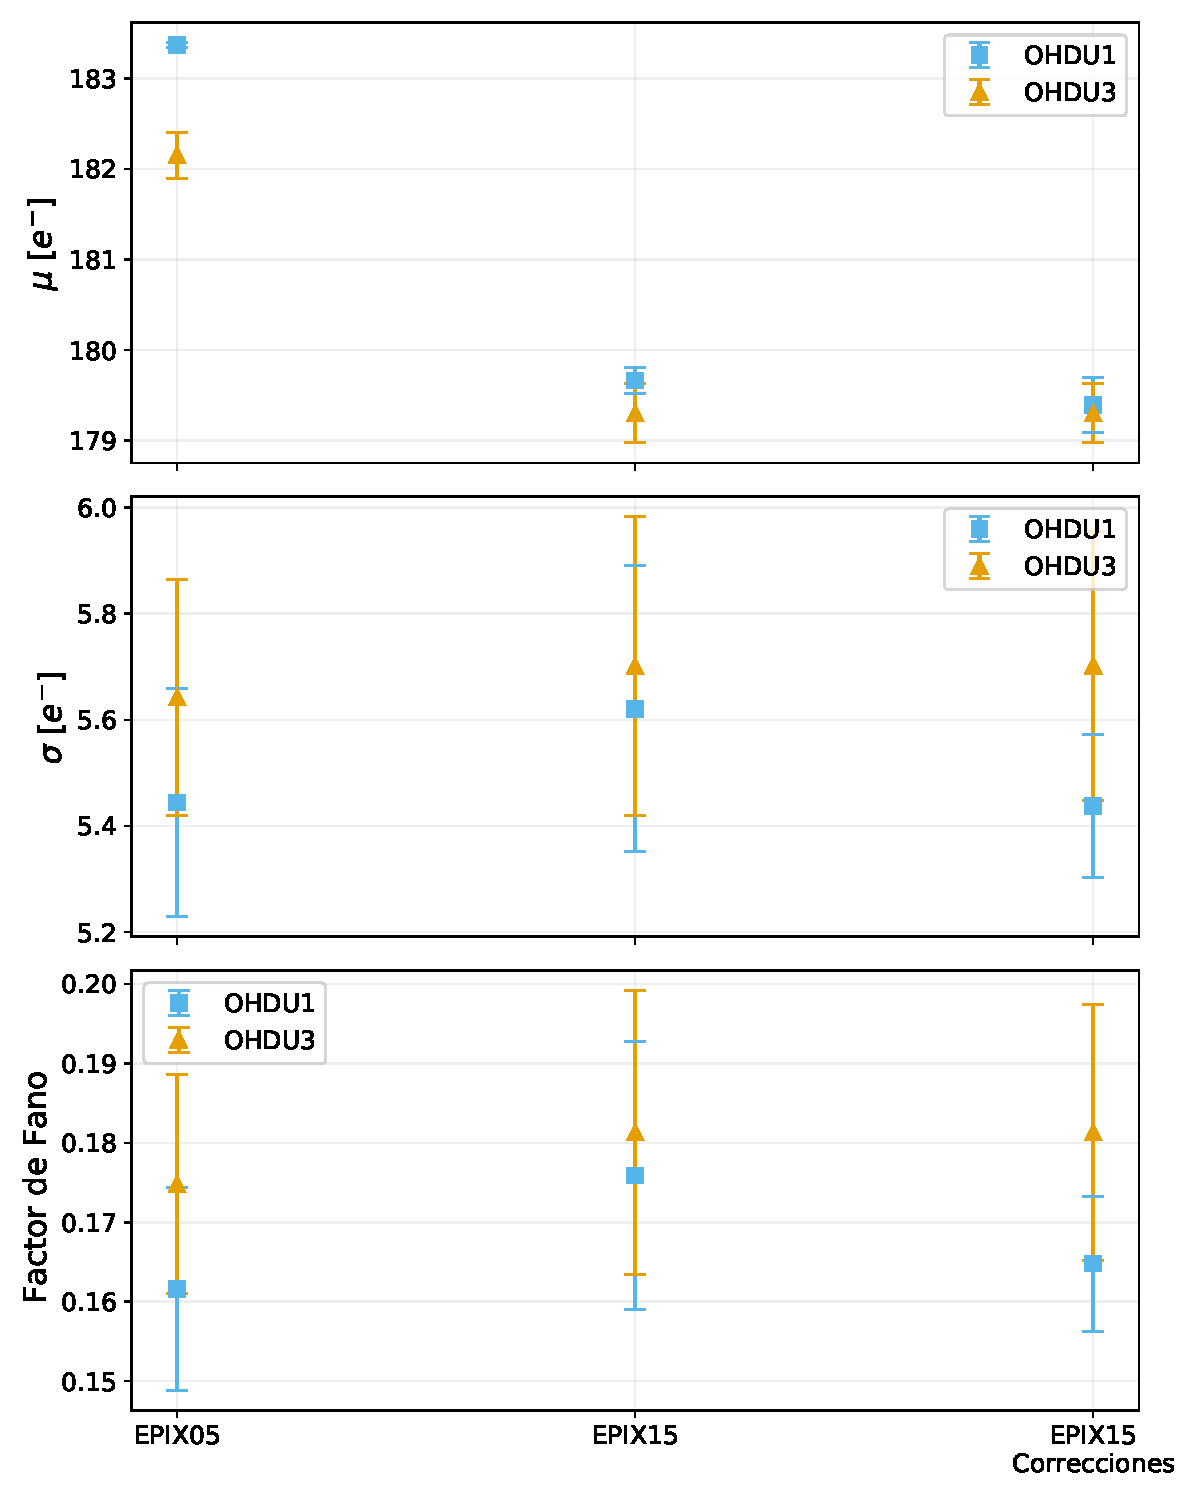
\includegraphics[scale=0.5]{Figs/F_mu_sigma_fano.pdf}
    \caption{\footnotesize{asd.}}
    \label{fig:F_mu_sigma_fano}
\end{figure}

La energía de creación electrón-hueco, por su parte, aumentó al aplicar el umbral y luego de aplicar las correcciones se mantuvieron los valores y se solaparon los errores entre los cuadrantes.
\begin{figure}[h]
    \centering
        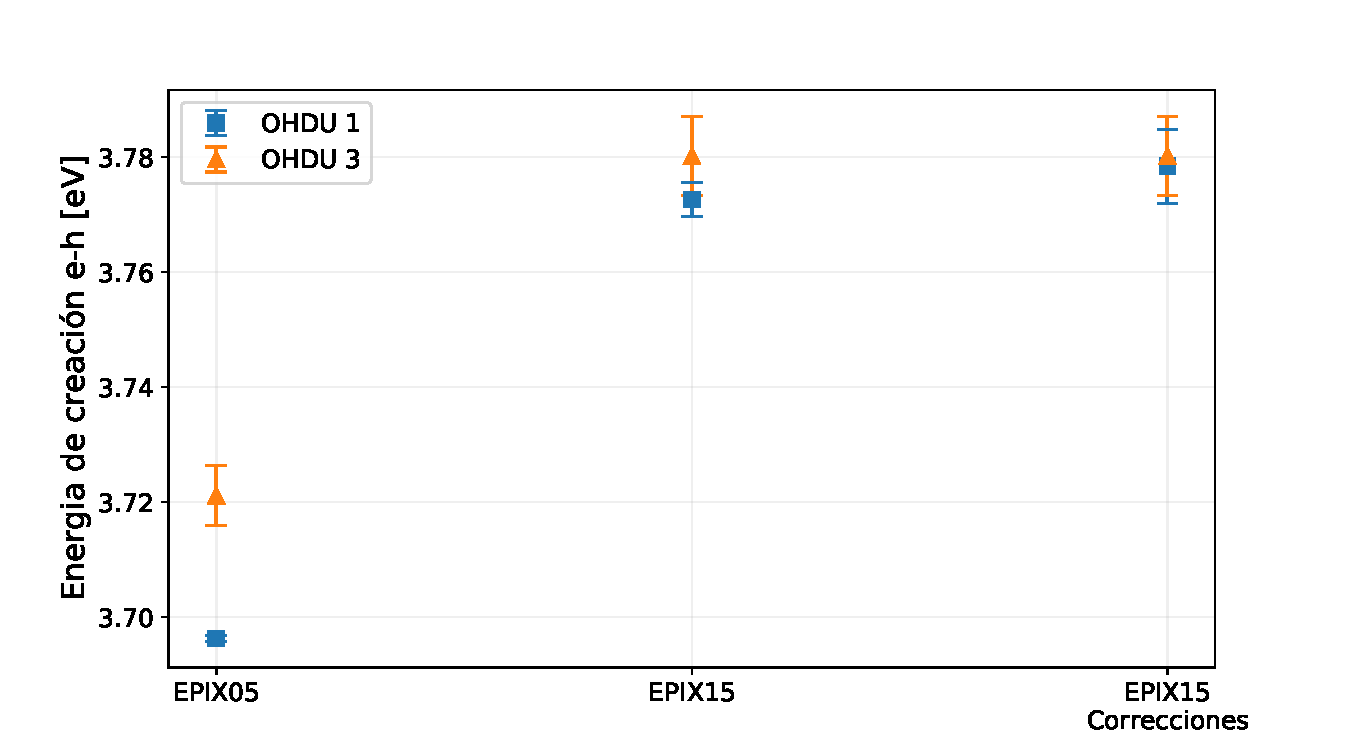
\includegraphics[scale=0.5]{Figs/F_energia_creacion_eh.pdf}
    \caption{\footnotesize{asd.}}
    \label{fig:F_energia_creacion_eh}
\end{figure}
%%%%%%%%%%%%%%%%%%%%%%%%%%%%%%%%%%%%%%%%%%%%%%%%%%%%%%%%%%%%%%%%%%
%%%%%%%%%%%%%%%%%%%%%%%%%%%%%%%%%%%%%%%%%%%%%%%%%%%%%%%%%%%%%%%%%%

%También se logra observar lo que se esperaba respecto a la intensidad de del parámetro $\beta$: Para los picos de los rayos $X$ del flúor, las colas en los picos de los histogramas son apreciablemente más pronunciadas que para los picos de los rayos $X$ del aluminio. Esto se debe a que $\beta_{F} = 0.008$ mientras que $\beta_{Al} = 0.001$, siendo el efecto de la PCC 8 veces más pronunciado para el caso del flúor.

% \begin{figure}[H]
%     \centering
%         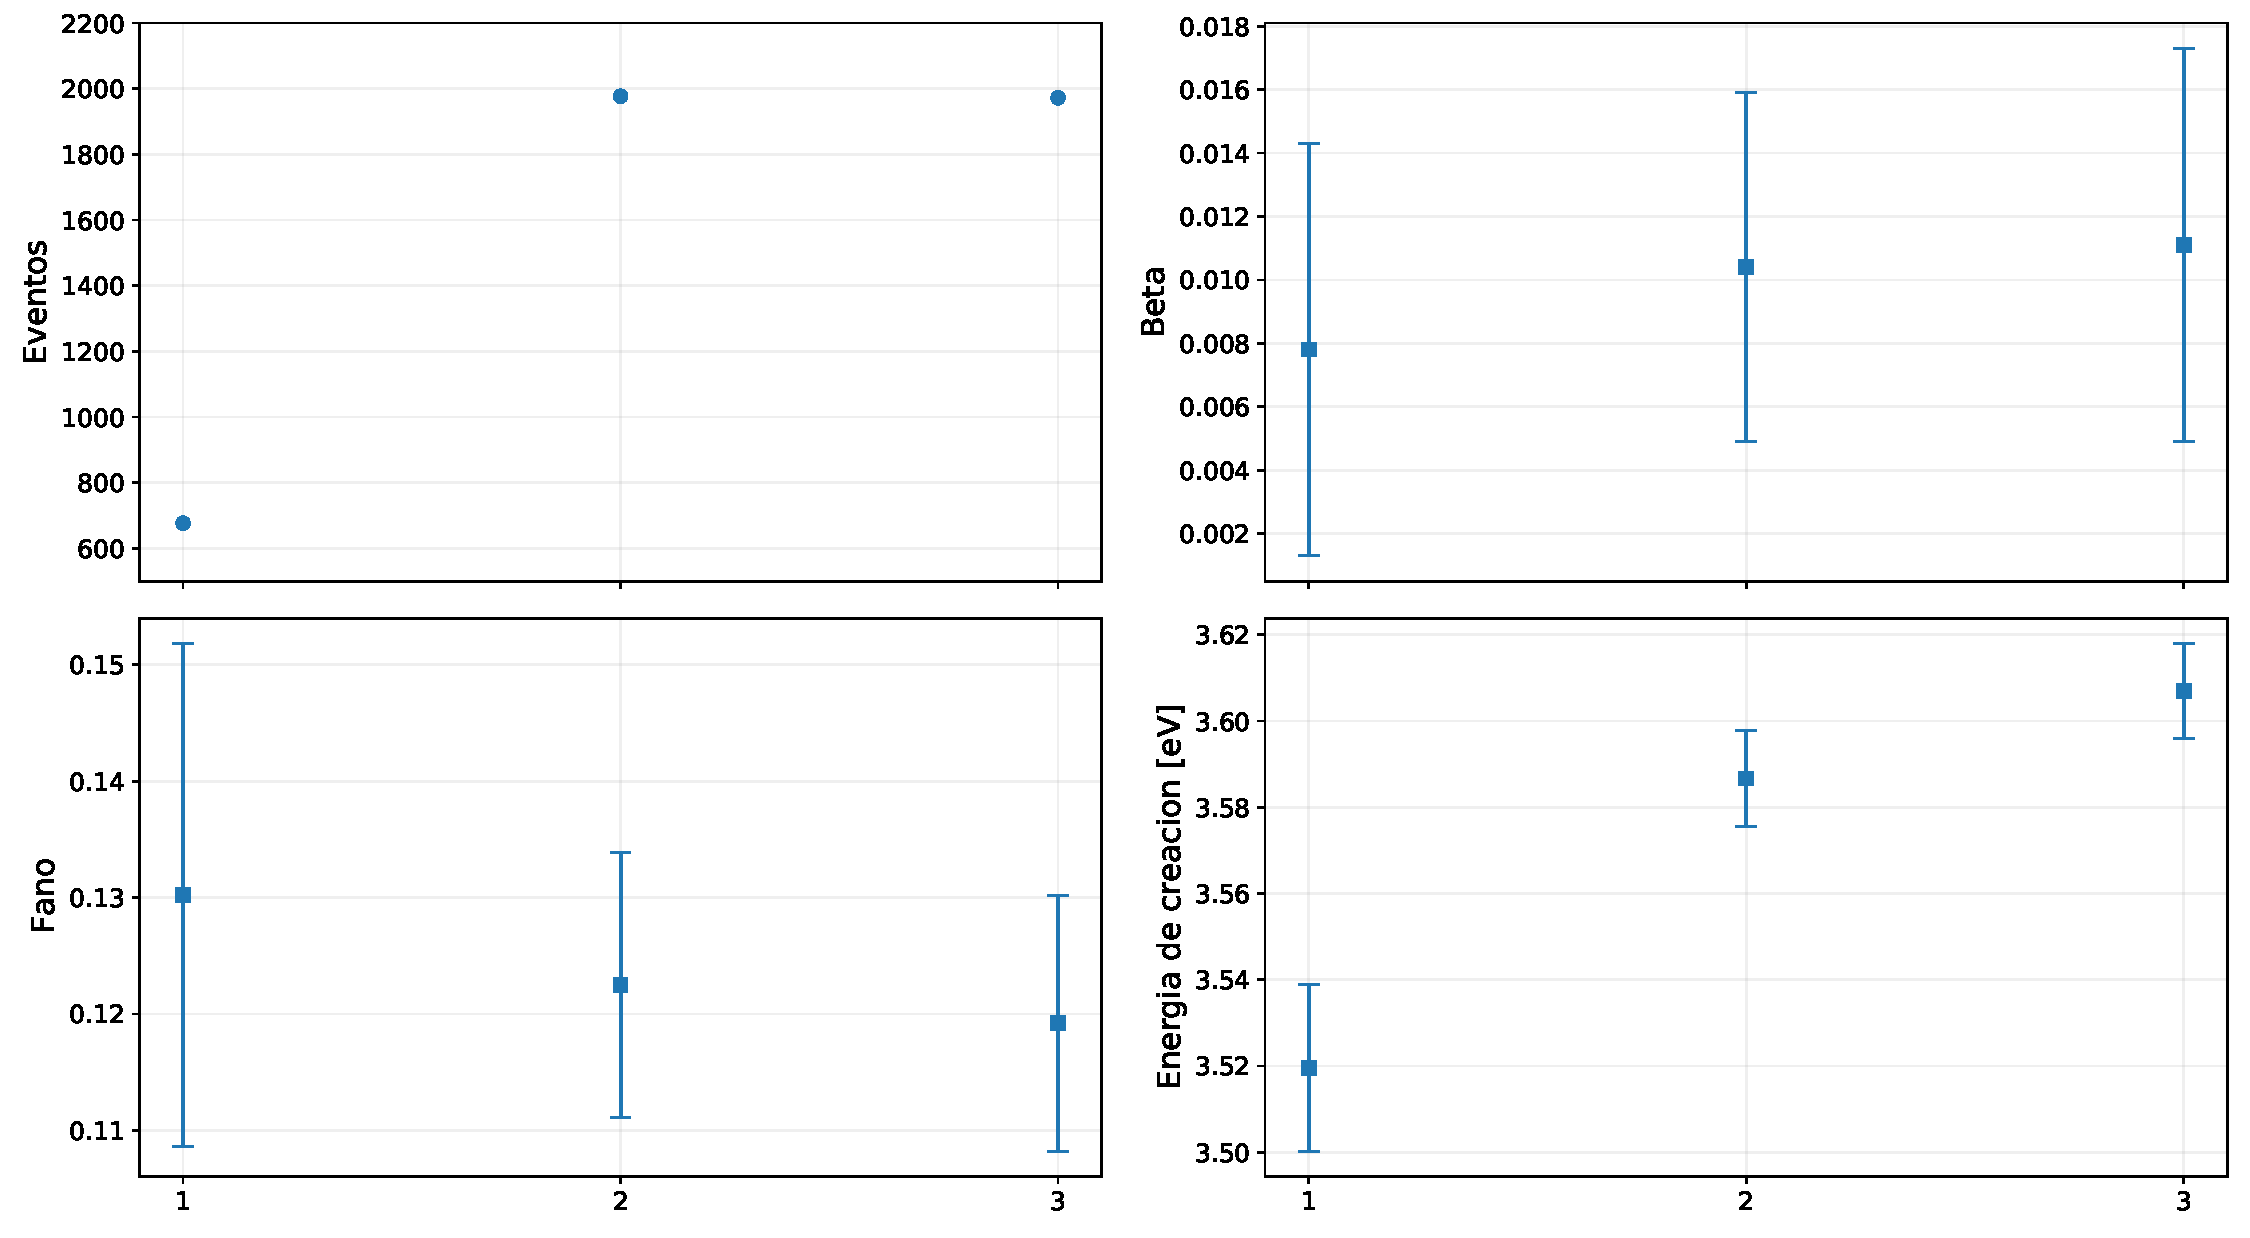
\includegraphics[scale=0.45]{Figs/F_OHDU1_EventosBetaFanoEH.pdf}
%     \caption{\footnotesize{Resultados para cada uno de los pasos de análisis para el flúor y el primer cuadrante. Se presentan la cantidad de eventos registrados, el valor del parámetro $\beta$, el factor de Fano y la energía de creación electrón hueco. AGREGAR QUE SIGNIFICA 1, 2, Y 3}}
%     \label{fig:F_OHDU1_EventosBetaFanoEH}
% \end{figure}
% \textcolor{red}{EL BETA NO IMPORTA, IMPORTA EL TAMAÑO DE LA PCC $\beta\tau_{CCE}$}
% ENERGIA DE CREACIÓN HUECO, FANO Y TAU (tamaño de la pcc) en un gráfico de $1x3$ (uno arriba del otro, no apaisado)
% \begin{figure}[H]
%     \centering
%         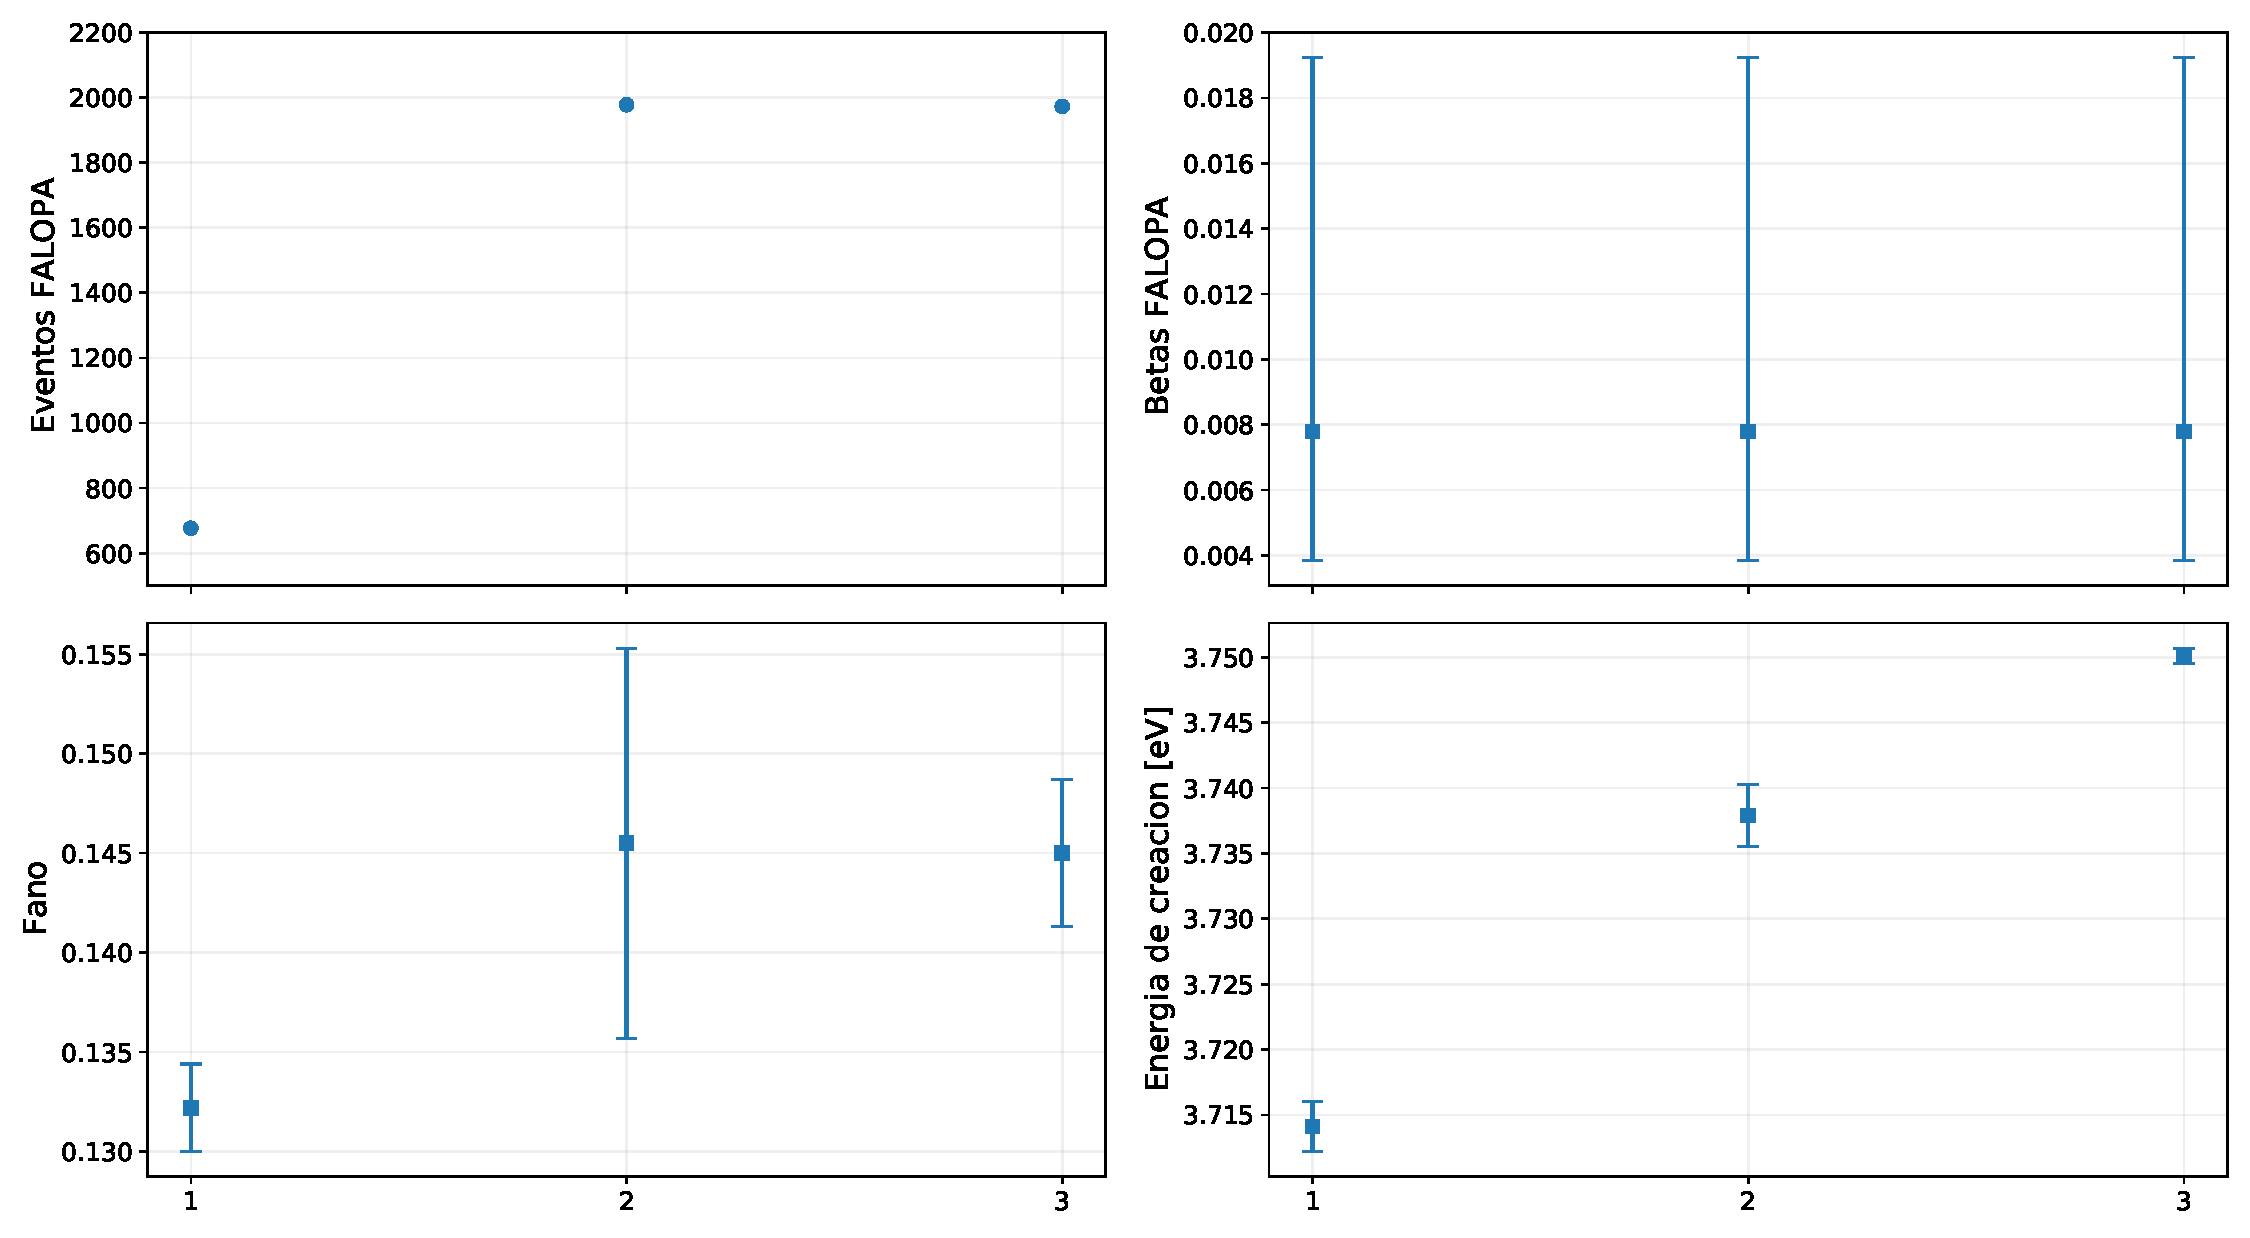
\includegraphics[scale=0.45]{Figs/Al_OHDU1_EventosBetaFanoEH.pdf}
%     \caption{\footnotesize{Resultados para cada uno de los pasos de análisis para el aluminio y el primer cuadrante. Se presentan la cantidad de eventos registrados, el valor del parámetro $\beta$, el factor de Fano y la energía de creación electrón hueco.\textcolor{red}{Acá puse la misma cantidad de eventos que los del flúor, porque los del aluminio no los tengo, no sé qué parte del codigo los printea en pantalla. También puse 3 veces el mismo valor de beta con sus intervalos porque no los tengo para el caso EPIX 0.5, EPIX 1.5 sin correcciones. En teoría este es para EPIX 1.5 con correcciones.}}}
%     \label{fig:Al_OHDU1_EventosBetaFanoEH}
% \end{figure}
%\noindent Primero sin aplicar el nuevo umbral, luego aplicando \verb|EPIX=1.5| sin correcciones y por último \verb|EPIX=1.5| con las correcciones, siempre tomando el primer cuadrante del sensor y finalmente resumiendo los resultados para los demás cuadrantes en una tablas.
%Para el primero de estos pasos puede verse el histograma de carga y su respectivo ajuste en la Figura \ref{fig:Al_OHDU1_EPIX05}, del cual se obtiene un valor para el factor de Fano de $F = 0.1322 \pm 0.0022$ y la energía de creación electrón hueco $\varepsilon_{\eh} = 3.7141 \pm 0.0019$
%\begin{figure}[H]
%    \centering
%        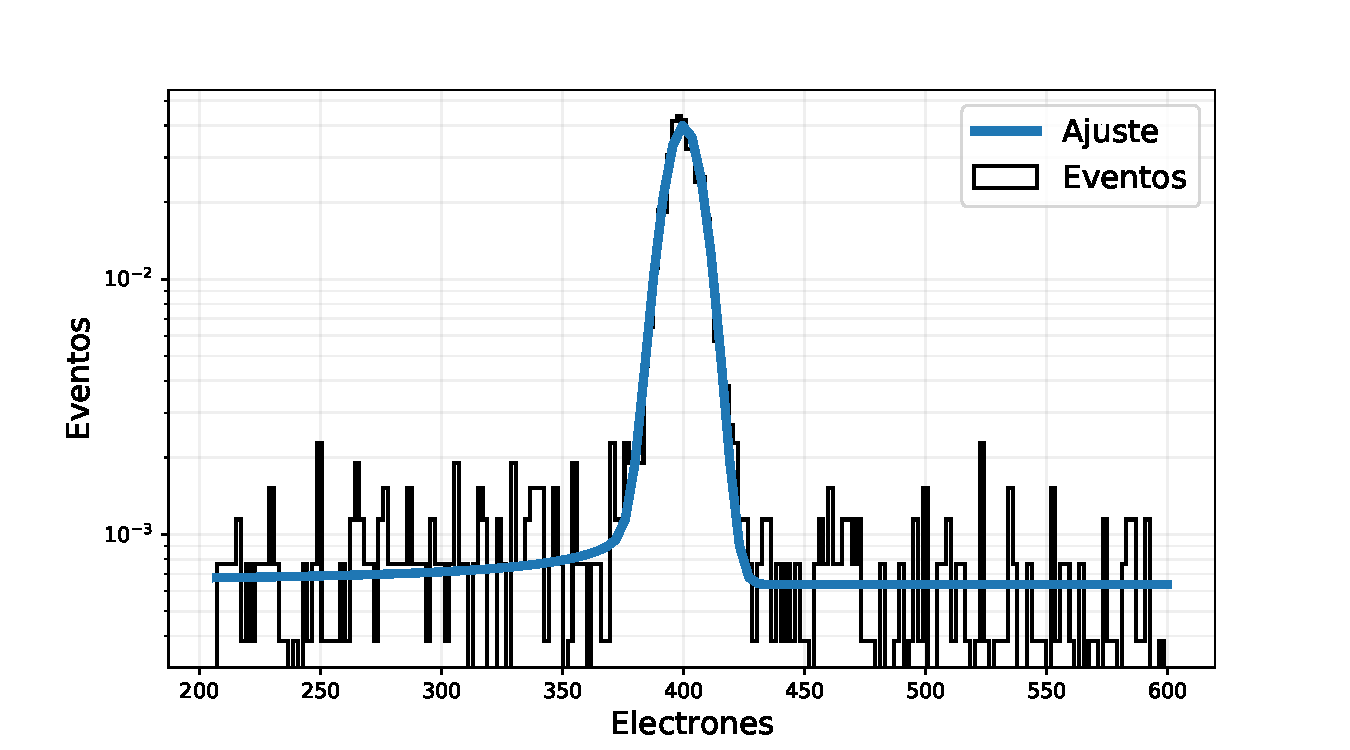
\includegraphics[scale=0.5]{Figs/HistFit_EPIX05_OHDU1_SinCorr.pdf}
%    \caption{\footnotesize{asd.}}
%    \label{fig:Al_OHDU1_EPIX05}
%\end{figure}

%El histograma y ajuste del pico del aluminio para el segundo paso del análisis se puede ver en la Figura \ref{fig:Al_OHDU1_EPIX15_SinCorr}. El valor del factor de Fano obtenido es $F = 0.1455 \pm 0.0098$ y para la energía de creación electrón-hueco $\varepsilon_{\eh} = 3.7379 \pm 0.0024$. Lo primero que se observa es que la incerteza del factor de Fano aumenta levemente lo cual es un resultado inesperado debido al aumento en la estadística luego de aplicar el umbral. Mismo caso para la energía de creación electrón hueco, donde la incerteza obtenida aumenta sutilmente. Los magnitudes también difieren entre sí más allá de sus errores, un $\sim 10\,\%$ para el factor de Fano y menos del $1\,\%$ para la energía de creación electrón hueco.
%\begin{figure}[H]
%    \centering
%        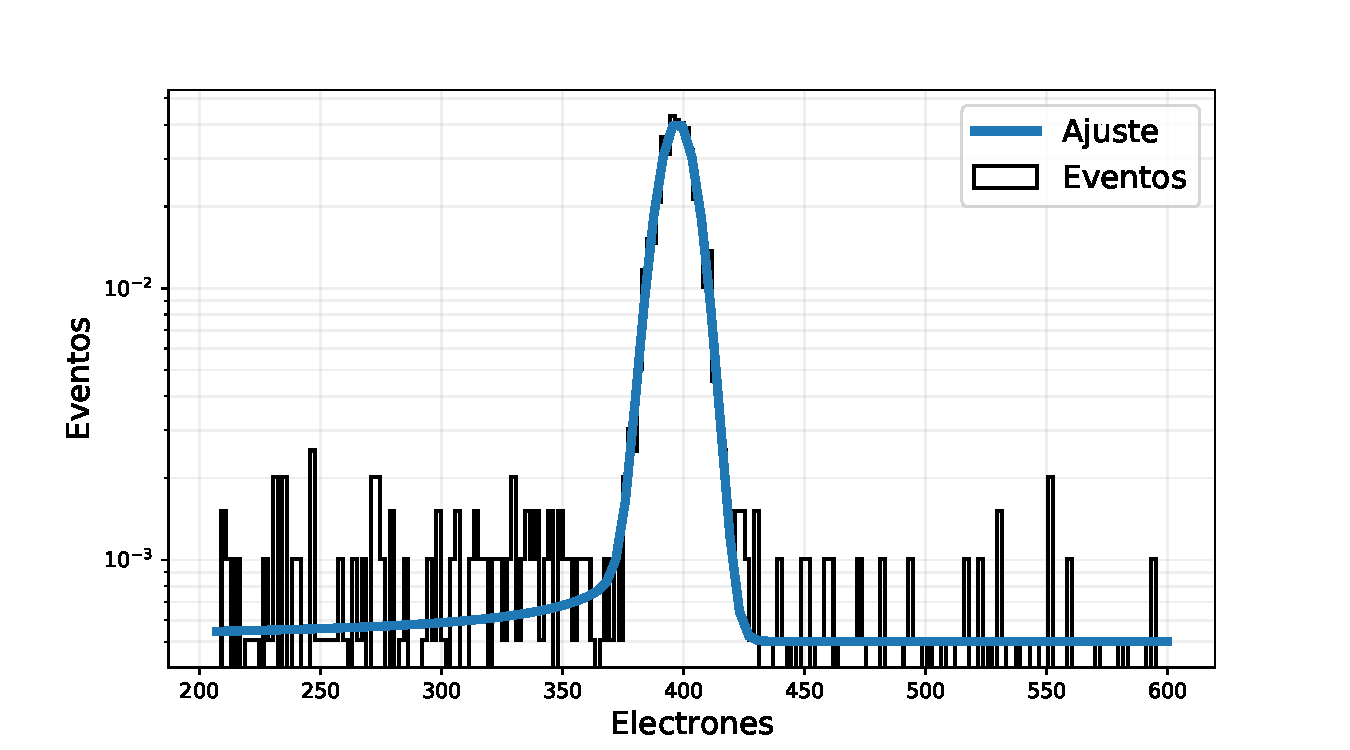
\includegraphics[scale=0.5]{Figs/HistFit_100c_EPIX15_OHDU1_SinCorr.pdf}
%    \caption{\footnotesize{asd.}}
%    \label{fig:Al_OHDU1_EPIX15_SinCorr}
%\end{figure}

%Por último, cuando se aplican tanto el umbral \verb|EPIX=1.5| como las correcciones en el programa y se generan los ajustes a los histogramas de carga, se obtiene que el factor de Fano es $F = 0.1450 \pm 0.0037$ y la energía de creación electrón hueco $\varepsilon_{\eh} = 3.7501 \pm 0.0006$. En efecto, se obtienen ligeras variaciones en los valores para el factor de Fano y la energía de creación electrón hueco. En cuanto a las incertezas, estas disminuyen bastante respecto a las anteriormente calculadas y, en particular, la incerteza de la energía de creación electrón hueco es demasiado pequeña.

%Al igual que para el caso del flúor, en las Tablas \ref{tab:FanoEehOHDU1y2} y \ref{tab:FanoEehOHDU3y4} se condensan los resultados obtenidos para los demás cuadrantes.

%Es importante destacar que para el caso del aluminio, no se observan diferencias apreciables en los ajustes para los diferentes análisis realizados sobre los datos. Por otro lado, también resulta relevante notar la diferencia en el efecto de la colección parcial de carga entre el flúor y el aluminio, donde para el primero las colas a la izquierda del pico son mucho más pronunciadas que para el aluminio. Esto se debe a que el valor de $\beta$ para el flúor resulta aproximadamente $8$ veces mayor que para el aluminio, con lo cual, hay mucha más carga que sufre recombinación producto de la PCC.


%\begin{table}[H]
% %\centering
% \begin{tabular}{@{}ccccc@{}}
% \toprule
%                 & \multicolumn{2}{c}{OHDU1}                 & \multicolumn{2}{c}{OHDU2}                 \\ \hline\hline
%                 & $F$                 & $\varepsilon_{\eh}$ & $F$                 & $\varepsilon_{\eh}$ \\
% EPIX 0.5 & $0.1322 \pm 0.0022$ & $3.7141 \pm 0.0019$ & $0.1401 \pm 0.0117$ & $3.7149 \pm 0.0037$ \\ \hline
% EPIX 1.5 50c & $0.1418 \pm 0.0148$ & $3.7399 \pm 0.0044$ & $0.1339 \pm 0.0186$ & $3.7532 \pm 0.0059$ \\
% EPIX 1.5 100c & $0.1455 \pm 0.0098$ & $3.7379 \pm 0.0024$ & $0.1530 \pm 0.0000$ & $3.7386 \pm 0.000$ \\ \hline
% EPIX 1.5 50c Corr & $0.1406 \pm 0.0000$ & $3.7490 \pm 0.0000$ & $0.1353 \pm 0.0187$ & $3.7421 \pm 0.0059$ \\
% EPIX 1.5 100c Corr & $0.1450 \pm 0.0037$ & $3.7501 \pm 0.0006$ & $0.1513 \pm 0.2640$ & $3.7270 \pm 0.0799$ \\ \bottomrule \hline
% \end{tabular}
% \caption{tabla}
% \label{tab:FanoEehOHDU1y2}
% \end{table}
% \begin{table}[H]
% \centering
% \begin{tabular}{@{}ccccc@{}}
% \toprule
%                 & \multicolumn{2}{c}{OHDU3}                 & \multicolumn{2}{c}{OHDU4}                 \\ \hline\hline
%                 & $F$                 & $\varepsilon_{\eh}$ & $F$                 & $\varepsilon_{\eh}$ \\
% EPIX 0.5 & $0.1498 \pm 0.00101$ & $3.7209 \pm 0.0029$ & $0.1812 \pm 0.0166$ & $3.7305 \pm 0.0041$ \\ \hline
% EPIX 1.5 50c & $0.1548 \pm 0.0001$ & $3.7449 \pm 0.0000$ & $0.1601 \pm 0.3691$ & $3.7633 \pm 0.1139$ \\
% EPIX 1.5 100c & $0.1699 \pm 0.0150$ & $3.7419 \pm 0.0039$ & $0.1931 \pm 0.0208$ & $3.7541 \pm 0.0000$ \\ \hline
% EPIX 1.5 50c  Corr& $0.1538 \pm 0.0000$ & $3.7510 \pm 0.0000$ & $0.1487 \pm 0.0000$ & $3.7698 \pm 0.0000$ \\
% EPIX 1.5 100c Corr& $0.1701 \pm 0.0141$ & $3.7485 \pm 0.0039$ & $0.1933 \pm 0.0194$ & $3.7634 \pm 0.0047$ \\ \bottomrule \hline
% \end{tabular}
% \caption{tabla}
% \label{tab:FanoEehOHDU3y4}
% \end{table}


% \noindent Para el caso del pico del flúor, se tiene en el gráfico de la Figura \ref{fig:F_OHDU0_EPIX05} el ajuste del histograma de carga con \verb|EPIX=0.5|. Se puede observar como el modelo ajusta muy bien los datos. Además es importante destacar la cantidad de eventos que contabilizó el algoritmo de clusterización (\verb|skExtract|) fue $2379$. 
% \begin{figure}[h]
%     \centering
%         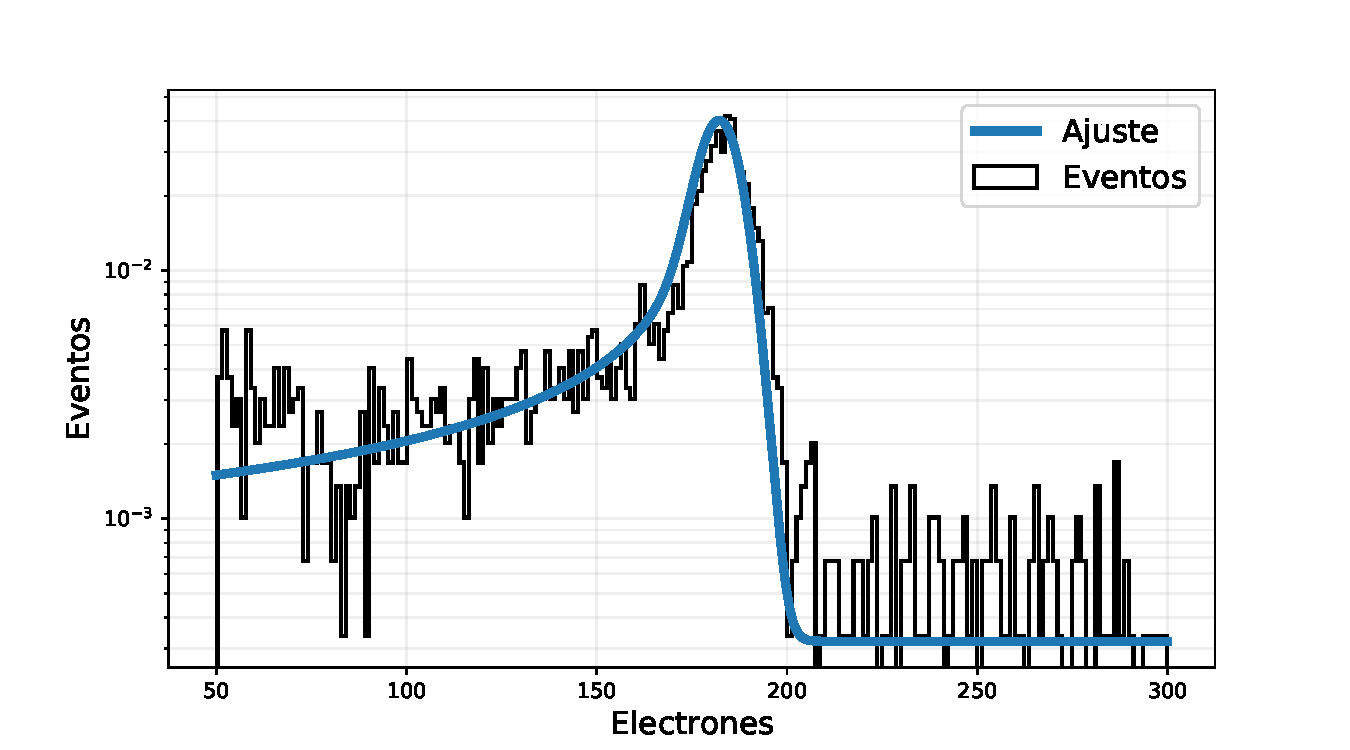
\includegraphics[scale=0.5]{Figs/HistFit_F_EPIX05_OHDU1.pdf}
%     \caption{\footnotesize{\textbf{completar}}}
%     \label{fig:F_OHDU0_EPIX05}
% \end{figure}
% De este ajuste se desprenden los valores de los parámetros de interés que son $\beta = 0.0078 \pm 0.0065$, el factor de Fano $F = 0.1480 \pm 0.0123$ y la energía de creación electrón hueco $\varepsilon_{\eh} = 3.6948 \pm 0.0054$.

% El segundo paso del análisis se muestra en el gráfico de la Figura \ref{fig:F_OHDU0_EPIX15conCorr}, donde se encuentra el ajuste de los datos para el caso en el que se utilizó el umbral \verb|EPIX=1.5| sin aplicar correcciones. El conteo de eventos en este caso fue de $1812$.
% \begin{figure}[h]
%     \centering
%         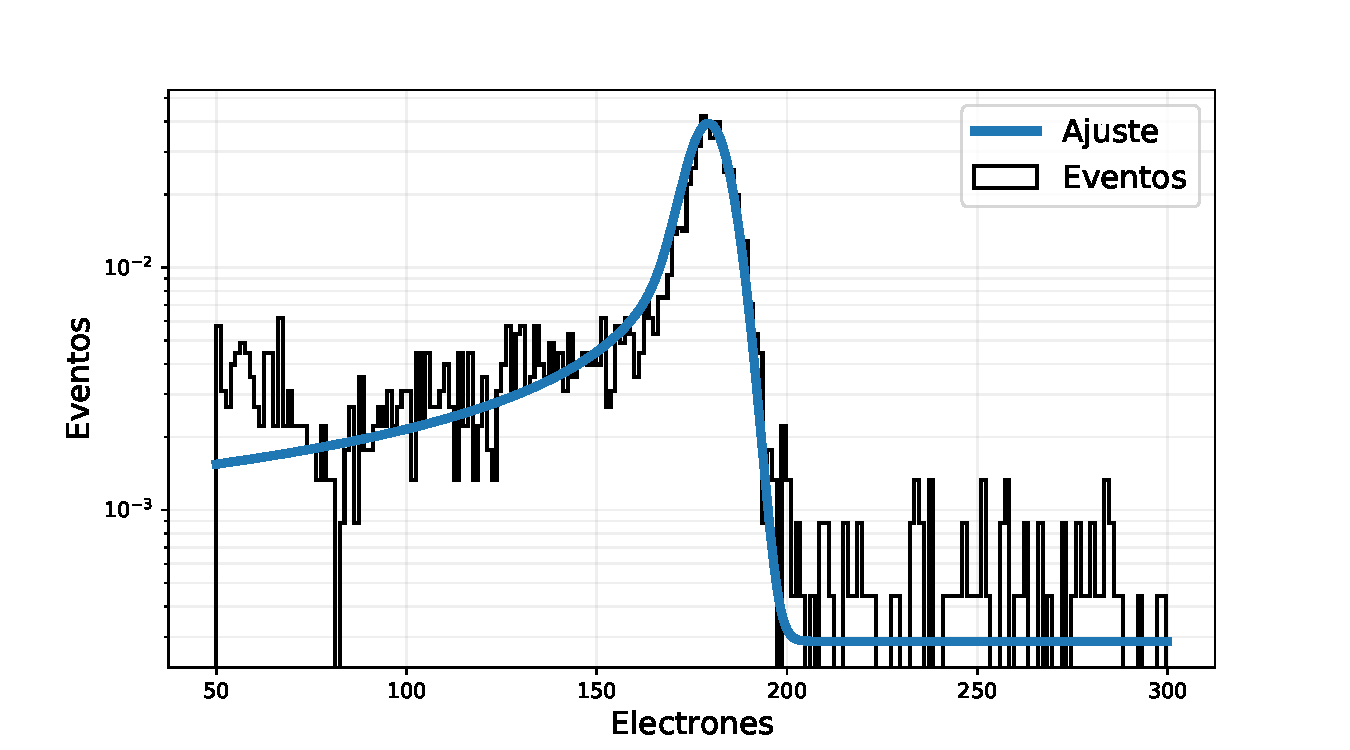
\includegraphics[scale=0.5]{Figs/HistFit_F_EPIX15_OHDU1.pdf}
%     \caption{\footnotesize{\textbf{completar}}}
%     \label{fig:F_OHDU0_EPIX15sinCorr}
% \end{figure}
% En este caso se tiene un apreciable aumento de $\beta$, obteniéndose $\beta = 0.0104 \pm 0.0055$, lo cual también es apreciable en el gráfico porque se observa mayor incidencia de eventos en la cola izquierda del pico. El factor de Fano resultó $F = 0.1553 \pm 0.0159$ y la energía de creación electrón hueco $\eh = 3.7516 \pm 0.0079$. Las incertezas de todos estos parámetros se redujeron sensiblemente respecto al caso anterior con menor estadística. Para el caso de los valores de los parámetros, el factor de Fano disminuyó, mientras que la energía de creación electrón hueco aumentó.

% En el tercer paso, utilizando \verb|EPIX=1.5| y las correcciones obtenidas de los análisis previos, se obtuvo el ajuste que se ven el gráfico de la Figura \ref{fig:F_OHDU0_EPIX15conCorr}. Este es muy similar al anterior, dado que el cambio más significativo es el aumento en la estadística mientras que las correcciones no introducen cambios visibles en los histogramas. El conteo de eventos resultó sutilmente menor al caso anterior, $1806$ lo cual resulta \textbf{inesperadoooooo}

% En cuanto a los parámetros, el valor del $\beta$ aumentó sensiblemente respecto al caso sin correciones, teniéndose $\beta = 0.0111 \pm 0.0062$. El factor de Fano disminuyó aún más, siendo $F = 0.1535 \pm 0.0157$ donde también disminuyó su incerteza. La energía de creación electrón hueco por su parte aumentó siendo $\varepsilon_{\eh} = 3.7744 \pm 0.0076$ y su incerteza también aumento ligeramente respecto al caso sin correciones.

% Los resultados de estos mismos análisis para el resto de los cuadrantes se condensas en las Tablas \ref{tab:F_FanoEehOHDU1y2} y \ref{tab:F_FanoEehOHDU3y4}

% \begin{table}[H]
% \centering
% \begin{tabular}{@{}ccccc@{}}
% \toprule
%                 & Eventos                 & $\beta$ & $F$                 & $\varepsilon_{\eh}$ \\ \hline \hline
% EPIX 0.5 & $677$ & $0.0078 \pm 0.0065$ & $0.1302 \pm 0.0216$ & $3.5195 \pm 0.0193$  \\
% EPIX 1.5 & $1977$ & $0.0104 \pm 0.0055$ & $0.1225 \pm 0.0114$ & $3.5867 \pm 0.0111$\\
% EPIX 1.5 Corr & $1972$ & $0.0111 \pm 0.0062$ & $0.1192 \pm 0.0110$ & $3.6069 \pm 0.0113$ \\ \bottomrule
% \end{tabular}
% \caption{tabla}
% \label{tab:F_FanoEehBetaEventos}
% \end{table}


% \begin{table}[H]
% \centering
% \begin{tabular}{@{}ccccc@{}}
% \toprule
%                 & \multicolumn{2}{c}{OHDU1}                 & \multicolumn{2}{c}{OHDU2}                 \\ \hline\hline
%                 & $F$                 & $\varepsilon_{\eh}$ & $F$                 & $\varepsilon_{\eh}$ \\
% EPIX 0.5 & $0.1302 \pm 0.0216$ & $3.5195 \pm 0.0193$ & $0.xxxx \pm 0.xxxx$ & $3.xxxx \pm 0.xxxx$ \\
% EPIX 1.5 & $0.1225 \pm 0.0114$ & $3.5867 \pm 0.0111$ & $0.xxxx \pm 0.xxxx$ & $3.xxxx \pm 0.xxxx$ \\
% EPIX 1.5 Corr & $0.1192 \pm 0.0110$ & $3.6069 \pm 0.0113$ & $0.xxxx \pm 0.xxxx$ & $3.xxxx \pm 0.xxxx$ \\ \bottomrule
% \end{tabular}
% \caption{tabla}
% \label{tab:F_FanoEehOHDU1y2}
% \end{table}


% \begin{table}[H]
% \centering
% \begin{tabular}{@{}ccccc@{}}
% \toprule
%                 & \multicolumn{2}{c}{OHDU3}                 & \multicolumn{2}{c}{OHDU4}                 \\ \hline\hline
%                 & $F$                 & $\varepsilon_{\eh}$ & $F$                 & $\varepsilon_{\eh}$ \\
% EPIX 0.5 & $0.xxxx \pm 0.xxxx $ & $3.xxxx \pm 0.xxxx $ & $0.xxxx \pm 0.xxxx $ & $3.xxxx \pm 0.xxxx $ \\ 
% EPIX 1.5 & $0.xxxx \pm 0.xxxx $ & $3.xxxx \pm 0.xxxx $ & $0.xxxx \pm 0.xxxx $ & $3.xxxx \pm 0.xxxx $ \\ 
% EPIX 1.5 Corr& $0.xxxx \pm 0.xxxx $ & $3.xxxx \pm 0.xxxx$ & $0.xxxx \pm 0.xxxx $ & $3.xxxx \pm 0.xxxx $ \\ \bottomrule
% \end{tabular}
% \caption{tabla}
% \label{tab:F_FanoEehOHDU3y4}
% \end{table}